\chapter{Waves}

%
%  SECTION 5.1 - Gravity and Capillary Waves
%

% 5.1.1 - Surface Waves (examples of waves, generation of surface waves, gravity and capillary waves and both combined, drawing of a wave and definitions)

\section{Surface Waves}

We turn our attention now to the \emph{interface} between two fluids -- in our discussion here, almost always this will be water and air.  In that case the interface is called a \emph{surface wave}.  Surface waves can be generated by wind, ocean tides, surface disturbances, and underwater disturbances (an earthquake, for example, giving rise to a tsunami).  Figure \ref{fig_pond} shows an example of wind-generated waves on a pond.  

\begin{figure}
\centering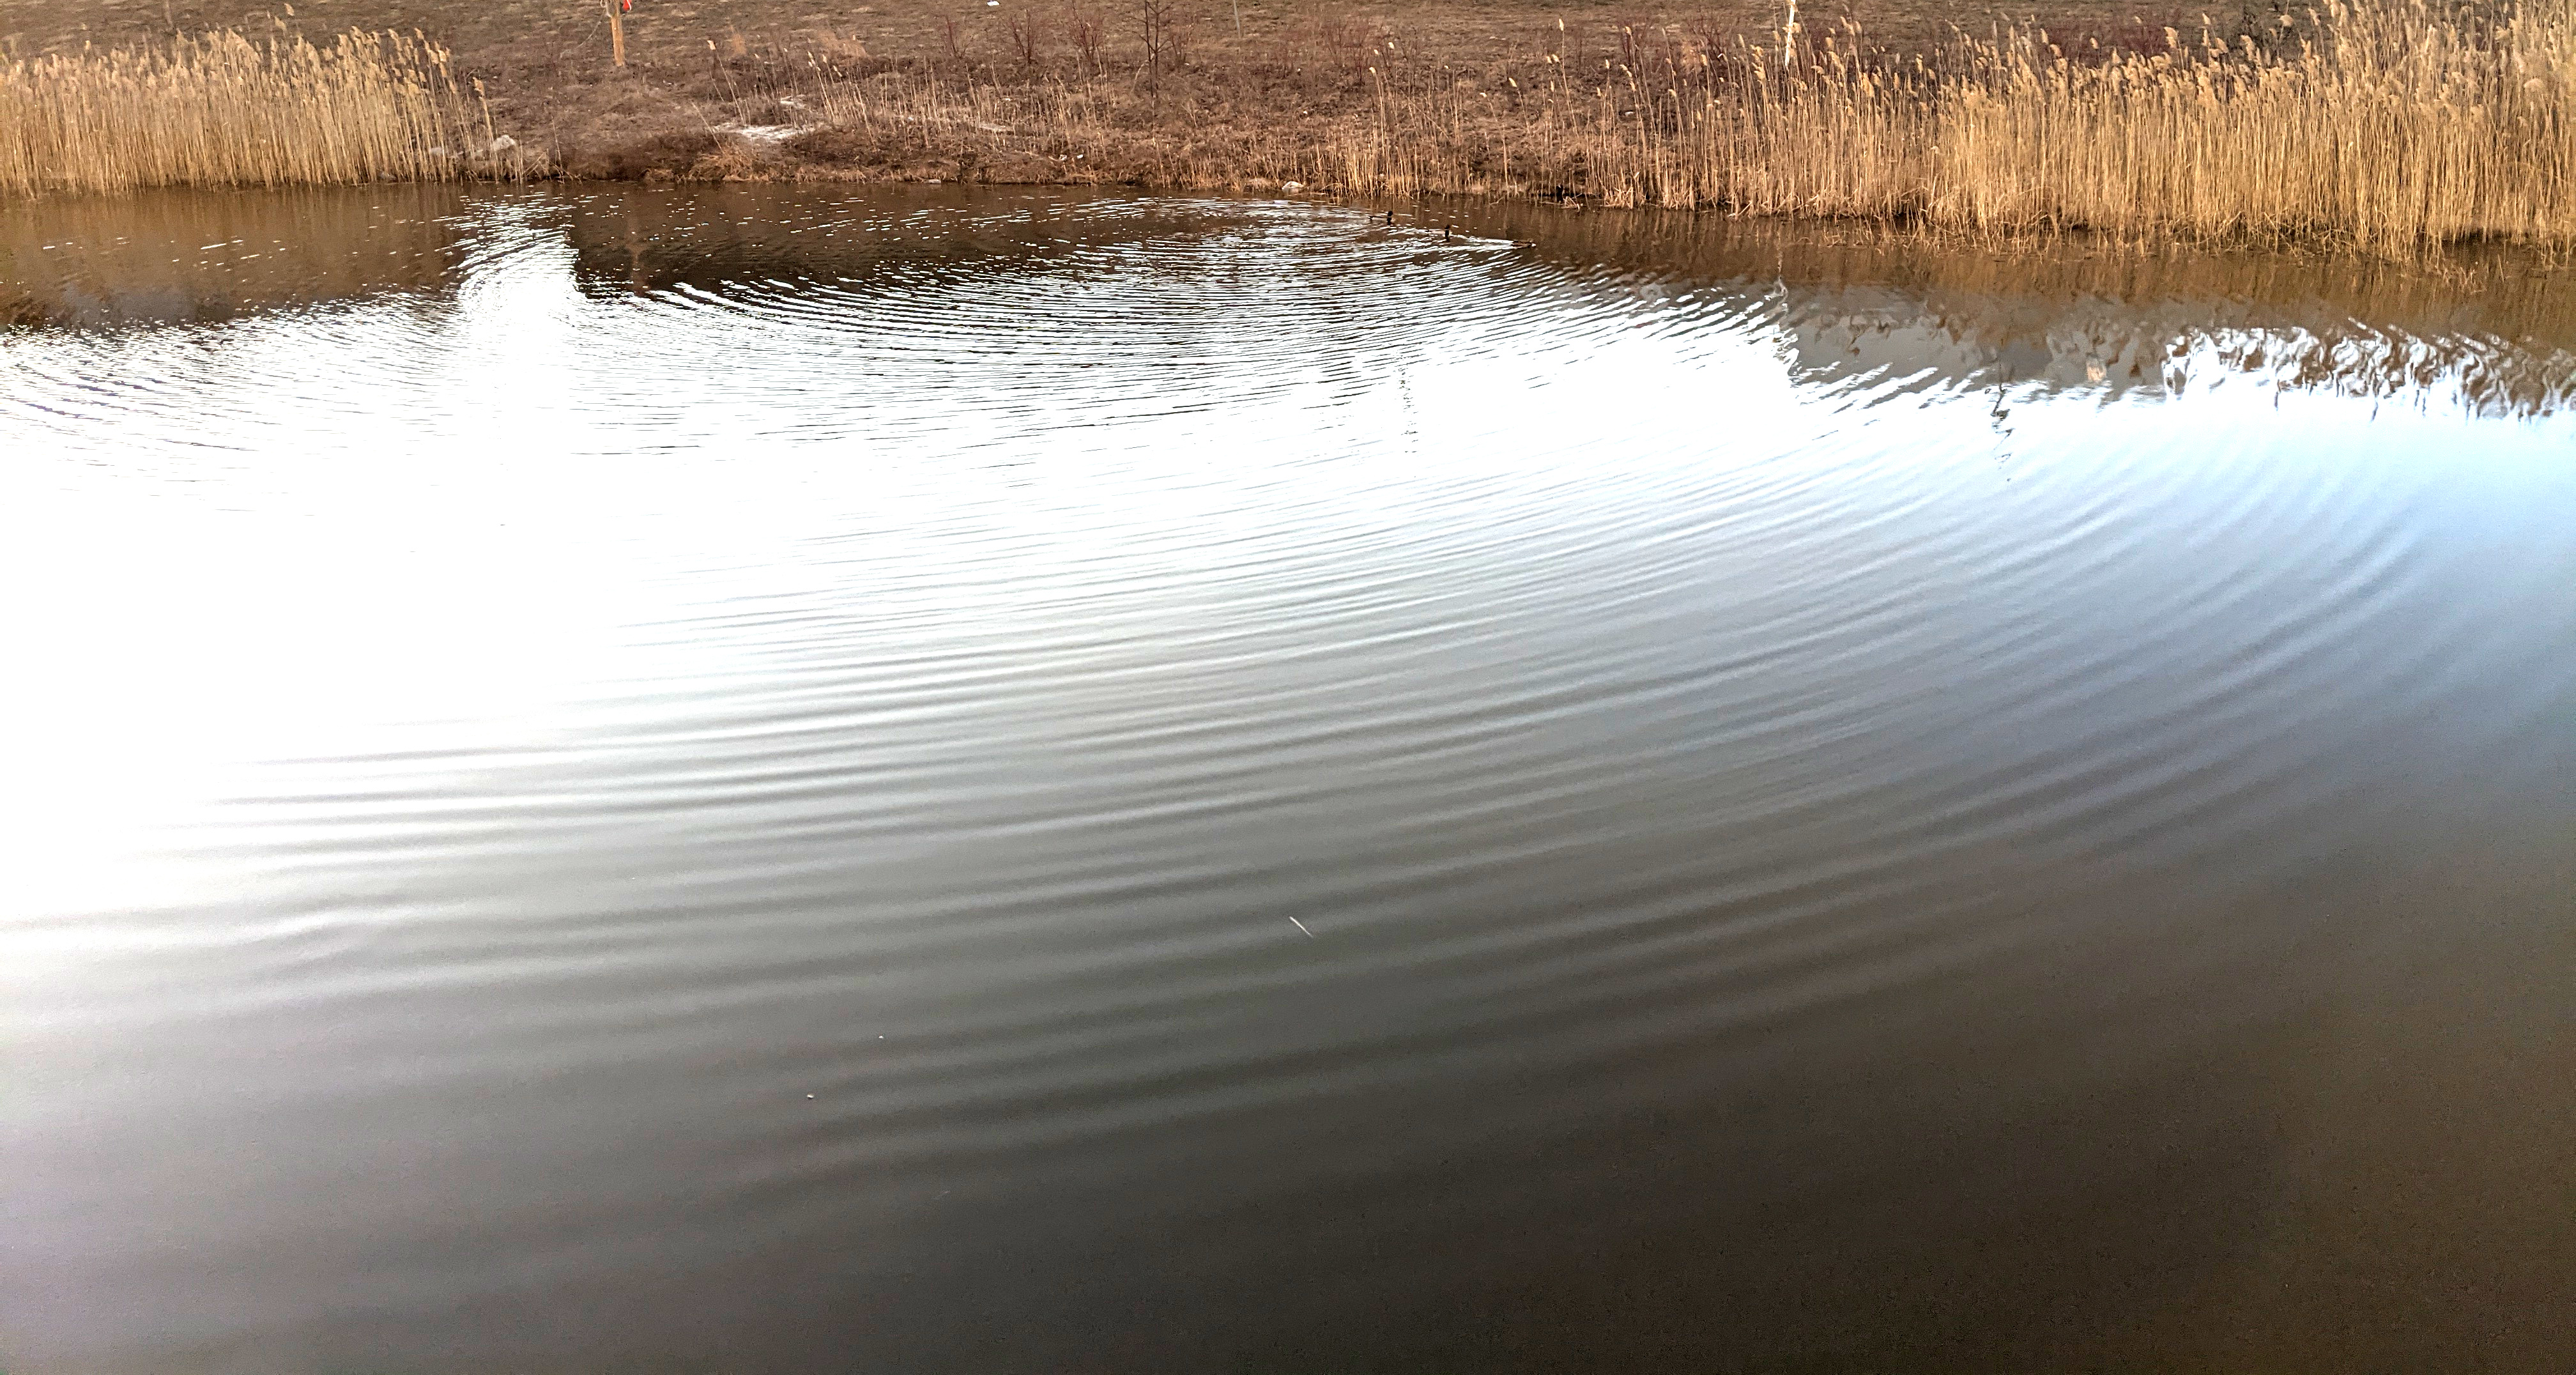
\includegraphics[width=0.9\linewidth]{Figures/Chapter5/fig_pond_waves}
\caption{Small amplitude waves generated by wind on the surface of a small pond on the cmapus of Ontario Tech University.}
\label{fig_pond}
\end{figure}

These waves are called \emph{gravity waves} since, as we'll see, the main force determining their behaviour is gravity.  However, in some cases -- typically when the wavelengths are very short -- \emph{surface tension} can be the dominant force in attempting to restore equilibrium to the surface.  In that case the waves can behave very differently, and often both forces are important in determining the dynamics of waves.

To begin our discussion of waves, consider a generic example of a surface wave as shown in Figure \ref{fig_generic_wave}.  The shape of the surface -- the interface between the two fluids -- will be described by the function $\eta(x, t)$, so that the surface itself is given by the equation
\begin{equation}
y = \eta(x, t).
\end{equation}
Note that we're setting the direction of gravity to be downward along the negative $y$ direction, in which case $\vec{g} = [0, -g, 0]$ in this coordinate system.

\begin{figure}
\centering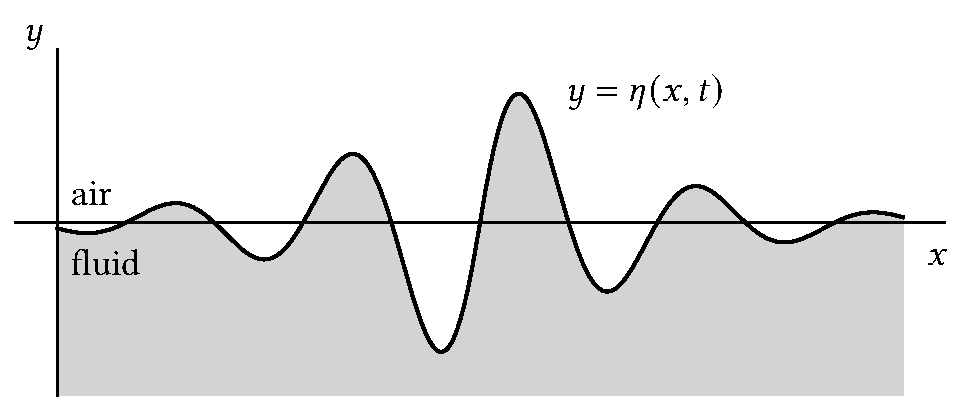
\includegraphics[width=0.9\linewidth]{Figures/Chapter5/fig_generic_wave}
\caption{The surface of a wave is described by the function $\eta(x, t)$.}
\label{fig_generic_wave}
\end{figure}

We'll assume that the fluid is two-dimensional, so there will be no $z$ dependence or flow in that direction:
\[
\vec{u} = [u(x, y, t), v(x, y, t), 0].
\]
We'll also take the flow to be irrotational, so that $\curl \vec{u} = \vec{0}$.  In two dimensions, this means
\[
\dfdx{v}{x} - \dfdx{u}{y} = 0.
\]
It might seem like a leap to assume irrotationality, but if we imagine starting with a perfectly still fluid, with no wave at the interface, then the flow is obviously initially irrotational.  But as time goes on, Kelvin's circulation theorem (see Section \ref{sec_circulation}) guarantees that the flow will remain irrotational -- the circulation must remain zero.

Since our flow is irrotational, we're free to describe it with the velocity potential $\varphi(x, y, t)$.  In two dimensions, $\vec{u} = \grad \varphi$ becomes
\begin{equation}
u = \dfdx{\varphi}{x} \quad \text{and} \quad \dfdx{\varphi}{y}.
\end{equation}
Finally, we're still dealing with incompressible fluids, which means the velocity potential must satisfy Laplace's equation:
\begin{equation}
\ddfdx{\varphi}{x} + \ddfdx{\varphi}{y} = 0.
\end{equation}
This lays out the guiding equations behind our discussion of waves; all that's left is to determine the boundary conditions.

% 5.1.2 - The Kinematic and Pressure Conditions

\section{The Kinematic and Pressure Conditions}

The first boundary condition comes from the fact that any fluid particle at the surface must remain at the surface.  You might be able to visualize this by imagining dyeing the fluid at the surface; as the surface moves up or down, the dyed fluid stays at the surface.  This means that those fluid particles at the surface must follow the vertical motion of the wave.  We can model this mathematically by defining a new function, $F(x, y, t)$, such that
\begin{equation}
F(x, y, t) = y - \eta(x, t).
\end{equation}
Although in general $F$ can take on any value, all fluid particles at the surface have $F =$ constant -- namely, $F(x, y, t) = 0$ there since $y = \eta(x, t)$ defines our surface.

With the function $F$ constant at the surface, we can obviously write
\[
\frac{DF}{Dt} = 0 \quad \text{on} \quad y = \eta(x, t)
\]
or, expanding the material derivative,
\begin{equation}
\label{eq_kin_cond_md}
\dfdx{F}{t} + (\vec{u} \cdot \grad ) F = 0 \quad \text{on} \quad y = \eta(x, t).
\end{equation}
Now,
\[
\dfdx{F}{t} = \frac{\partial}{\partial t} \Bigl( y - \eta(x, t) \Bigr) = -\dfdx{\eta}{t}
\]
and
\[
(\vec{u} \cdot \grad) F = u \dfdx{F}{x} + v\dfdx{F}{y} = -u \dfdx{\eta}{x} + v,
\]
so equation (\ref{eq_kin_cond_md}) becomes
\[
-\dfdx{\eta}{t} - u\dfdx{\eta}{x} + v = 0,
\]
or
\begin{equation}
\label{eq_kin_cond}
\boxed{
\dfdx{\eta}{t} + u\dfdx{\eta}{x} = v \quad \text{on} \quad y = \eta(x, t).
}
\end{equation}
This is called the \emph{kinematic condition} at the surface; it ensures that fluid particles at the surface move vertically as the surface does.

The second boundary condition at the surface follows from considering the pressure in the fluid:  it must be \emph{continuous} across the interface.  Since we're usually assuming air above the fluid, we'll take the pressure at the surface to be atmospheric pressure, $p_0$, which is of course constant along the surface.  

Consider Euler's equation in the form of equation \ref{eq_euler_bernoulli},
\[
\frac{\partial \uu}{\partial t} + (\curl \uu ) \times \uu = -\grad \left( \frac{p}{\rho} + \tfrac{1}{2} \uu^2 + \Phi \right).
\]
The second term on the left is zero here, since we have irrotational flow, and we can write $\vec{u} = \grad \varphi$ and then combine the velocity potential with the other terms in the gradient on the right.  We then have
\[
\grad \left( \dfdx{\varphi}{t} + \frac{p}{\rho} + \frac{1}{2} \vec{u}^2 + \Phi \right) = 0.
\]
Integrating leads to
\begin{equation}
\label{eq_euler_wave}
\dfdx{\varphi}{t} + \frac{p}{\rho} + \frac{1}{2} \vec{u}^2 + \Phi = G(t),
\end{equation}
where $G(t)$ is the integration ``constant'' -- it can still be a function of time.  But we're free to take $G(t)$ to be anything we want, since it will go away once we take the space derivative. So, for reasons we'll see in a second, let's take it to be
\begin{equation}
G(t) = \frac{p_0}{\rho}.
\end{equation}
Note that that's the constant atmospheric pressure $p_0$ in that equation.

Our next step is to evaluate equation (\ref{eq_euler_wave}) at the surface $y = \eta(x, t)$:
\[
\dfdx{\varphi}{t} + \frac{p_0}{\rho} + \frac{1}{2} \vec{u}^2 + \Phi = \frac{p_0}{\rho} \quad \text{on} \quad y = \eta(x, t).
\]
Now we see why that choice of $G(t)$ was made, since the pressure terms cancel out.  Writing $\Phi = gy$ and $\vec{u}^2 = u^2 + v^2$, this becomes
\begin{equation}
\label{eq_pressure_cond}
\boxed{
\dfdx{\varphi}{t} +  \frac{1}{2}(u^2 + v^2) + g\eta = 0 \quad \text{on} \quad y = \eta(x, t).
}
\end{equation}
This is the \emph{pressure condition}, the second boundary condition that must be satisfied by the wave surface.  Together with the kinematic condition and Laplace's equation, they make up the theory of surface waves.  Unfortunately, although Laplace's equation is linear, the boundary conditions are not, and this makes them rather difficult to work with.  


% 5.1.3 - Small Amplitude Waves (linearization)

\section{Small Amplitude Waves}


% 5.1.4 - Sinusoidal Waves (dispersion relation, potential, example of fluid path under wave)


% 5.1.5 - Capillary Waves (surface tension effects, new BCs, surface tension-dominated waves, etc; include pic of the two types of waves, plus downstream/upstream stuff and pic of that)


%
%  SECTION 5.2 - Group Waves
%

% 5.2.1 - Wave Packets

% 5.2.2 - Group Velocity


%
%  SECTION 5.3 - Sound waves
%

% 5.3.1 - Compressible Fluids

% 5.3.2 - Small Amplitude Sound waves


